%% This file was auto-generated by IPython.
%% Conversion from the original notebook file:
%% stat_hadoop_logreg.ipynb
%%
\documentclass[11pt,english,fleqn]{article}

%% This is the automatic preamble used by IPython.  Note that it does *not*
%% include a documentclass declaration, that is added at runtime to the overall
%% document.

\usepackage{amsmath}
\usepackage{amssymb}
\usepackage{graphicx}
\usepackage{ucs}
\usepackage[utf8x]{inputenc}

% needed for markdown enumerations to work
\usepackage{enumerate}

% Slightly bigger margins than the latex defaults
\usepackage{geometry}
\geometry{verbose,tmargin=3cm,bmargin=3cm,lmargin=2.5cm,rmargin=2.5cm}

% Define a few colors for use in code, links and cell shading
\usepackage{color}
\definecolor{orange}{cmyk}{0,0.4,0.8,0.2}
\definecolor{darkorange}{rgb}{.71,0.21,0.01}
\definecolor{darkgreen}{rgb}{.12,.54,.11}
\definecolor{myteal}{rgb}{.26, .44, .56}
\definecolor{gray}{gray}{0.45}
\definecolor{lightgray}{gray}{.95}
\definecolor{mediumgray}{gray}{.8}
\definecolor{inputbackground}{rgb}{.95, .95, .85}
\definecolor{outputbackground}{rgb}{.95, .95, .95}
\definecolor{traceback}{rgb}{1, .95, .95}

% Framed environments for code cells (inputs, outputs, errors, ...).  The
% various uses of \unskip (or not) at the end were fine-tuned by hand, so don't
% randomly change them unless you're sure of the effect it will have.
\usepackage{framed}

% remove extraneous vertical space in boxes
\setlength\fboxsep{0pt}

% codecell is the whole input+output set of blocks that a Code cell can
% generate.

% TODO: unfortunately, it seems that using a framed codecell environment breaks
% the ability of the frames inside of it to be broken across pages.  This
% causes at least the problem of having lots of empty space at the bottom of
% pages as new frames are moved to the next page, and if a single frame is too
% long to fit on a page, will completely stop latex from compiling the
% document.  So unless we figure out a solution to this, we'll have to instead
% leave the codecell env. as empty.  I'm keeping the original codecell
% definition here (a thin vertical bar) for reference, in case we find a
% solution to the page break issue.

%% \newenvironment{codecell}{%
%%     \def\FrameCommand{\color{mediumgray} \vrule width 1pt \hspace{5pt}}%
%%    \MakeFramed{\vspace{-0.5em}}}
%%  {\unskip\endMakeFramed}

% For now, make this a no-op...
\newenvironment{codecell}{}

 \newenvironment{codeinput}{%
   \def\FrameCommand{\colorbox{inputbackground}}%
   \MakeFramed{\advance\hsize-\width \FrameRestore}}
 {\unskip\endMakeFramed}

\newenvironment{codeoutput}{%
   \def\FrameCommand{\colorbox{outputbackground}}%
   \vspace{-1.4em}
   \MakeFramed{\advance\hsize-\width \FrameRestore}}
 {\unskip\medskip\endMakeFramed}

\newenvironment{traceback}{%
   \def\FrameCommand{\colorbox{traceback}}%
   \MakeFramed{\advance\hsize-\width \FrameRestore}}
 {\endMakeFramed}

% Use and configure listings package for nicely formatted code
\usepackage{listingsutf8}
\lstset{
  language=python,
  inputencoding=utf8x,
  extendedchars=\true,
  aboveskip=\smallskipamount,
  belowskip=\smallskipamount,
  xleftmargin=2mm,
  breaklines=true,
  basicstyle=\small \ttfamily,
  showstringspaces=false,
  keywordstyle=\color{blue}\bfseries,
  commentstyle=\color{myteal},
  stringstyle=\color{darkgreen},
  identifierstyle=\color{darkorange},
  columns=fullflexible,  % tighter character kerning, like verb
}

% The hyperref package gives us a pdf with properly built
% internal navigation ('pdf bookmarks' for the table of contents,
% internal cross-reference links, web links for URLs, etc.)
\usepackage{hyperref}
\hypersetup{
  breaklinks=true,  % so long urls are correctly broken across lines
  colorlinks=true,
  urlcolor=blue,
  linkcolor=darkorange,
  citecolor=darkgreen,
  }

% hardcode size of all verbatim environments to be a bit smaller
\makeatletter 
\g@addto@macro\@verbatim\small\topsep=0.5em\partopsep=0pt
\makeatother 

% Prevent overflowing lines due to urls and other hard-to-break entities.
\sloppy

\setlength{\mathindent}{0pt}
\setlength{\parindent}{0pt}
\setlength{\parskip}{8pt}
\begin{document}

Paralel Lojistik Regresyon, Hadoop

Lojistik regresyon kodunu esle-indirge (map-reduce) uzerinden paralelize
etmek icin literature {[}1-7{]} bakinca, genel yaklasimin makinalara
bolunen veri parcalari uzerinde ayri ayri grayan cikis (gradient ascent)
isletilmesi ve sonuc $\theta$'larin son bir makinada ortalamasinin
alinmasi oldugunu goruruz.

Daha onceki \emph{lojistik regresyon} yazimizda iki farkli gradyan cikis
algoritmasi gormustuk. Bu algoritmalardan kullanacagimiz daha basit
olani, her dongude alpha'yi degistiren, versiyon degil tek alpha
kullanan, ve kod icinde zar atan degil, veriyi sirayla isleyen. Bunun
birkac sebebi var, oncelikle altta gorecegimiz uzere veriyi Hadoop'a
vermeden once kendimiz karistiracagiz, yani kod icinde zar atmaya gerek
kalmayacak. Ikincisi pek cok makinada islem yapildigi icin tek bir sabit
uzerinden azaltma yapmak mumkun degil, bu sebeple ve basitlik amaciyla
tek sabitli kod kullanildi. Ayrica artik dongu (iterasyon) yok, yani
veri bastan sona bir kez tarandi mi, o makinanin islemi bitecek. Fakat
buyuk veri ortaminda (ki zaten onun icin Hadoop kullaniyoruz herhalde)
elimizde o kadar cok veri olacak ki bu verinin tamamini isleyince zaten
100,200 kere donguyu isletmek ile ayni etkiyi almis oluyoruz.

Ornek veri olarak alttakini urettik,

\begin{codecell}
\begin{codeinput}
\begin{lstlisting}
from pandas import *
\end{lstlisting}
\end{codeinput}
\end{codecell}
\begin{codecell}
\begin{codeinput}
\begin{lstlisting}
mean1 = [10,10]
mean2 = [20,20]
cov = [[5,0],[0,5]]
d1 = DataFrame(np.random.multivariate_normal(mean1,cov,10000))
d2 = DataFrame(np.random.multivariate_normal(mean2,cov,10000))
d1['labels'] = 1
d2['labels'] = 0
data = DataFrame(np.vstack((d1,d2)))
data.to_csv("testSet.txt",sep='\t',index=None,header=None)
print data[:4]
\end{lstlisting}
\end{codeinput}
\begin{codeoutput}
\begin{verbatim}
0          1  2
0   9.897078   9.232074  1
1  10.151486  11.126241  1
2   9.498804   7.898127  1
3   9.912641   9.688876  1
\end{verbatim}
\end{codeoutput}
\end{codecell}
\begin{codecell}
\begin{codeinput}
\begin{lstlisting}
plt.plot(d1.ix[:,0],d1.ix[:,1],'b.')
plt.hold(True)
plt.plot(d2.ix[:,0],d2.ix[:,1],'r.')
plt.hold(True)

\end{lstlisting}
\end{codeinput}
\begin{codeoutput}
\begin{center}
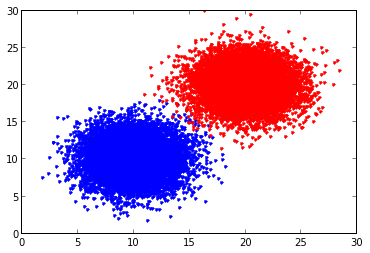
\includegraphics[width=0.7\textwidth]{stat_hadoop_logreg_files/stat_hadoop_logreg_fig_00.png}
\par
\end{center}
\end{codeoutput}
\end{codecell}
Hadoop'u baslatalim,

\begin{codecell}
\begin{codeinput}
\begin{lstlisting}
!ssh localhost -l hduser /home/hduser/Downloads/hadoop*/bin/stop-all.sh
!ssh localhost -l hduser /home/hduser/Downloads/hadoop*/bin/start-all.sh

\end{lstlisting}
\end{codeinput}
\begin{codeoutput}
\begin{verbatim}
stopping jobtracker
\end{verbatim}
\begin{verbatim}
localhost: stopping tasktracker
\end{verbatim}
\begin{verbatim}
stopping namenode
\end{verbatim}
\begin{verbatim}
localhost: stopping datanode
\end{verbatim}
\begin{verbatim}
localhost: stopping secondarynamenode
\end{verbatim}
\begin{verbatim}
starting namenode, logging to /home/hduser/Downloads/hadoop-1.0.4/libexec/../logs/hadoop-hduser-namenode-burak-Aspire-S3.out
\end{verbatim}
\begin{verbatim}
localhost: starting datanode, logging to /home/hduser/Downloads/hadoop-1.0.4/libexec/../logs/hadoop-hduser-datanode-burak-Aspire-S3.out
\end{verbatim}
\begin{verbatim}
localhost: starting secondarynamenode, logging to /home/hduser/Downloads/hadoop-1.0.4/libexec/../logs/hadoop-hduser-secondarynamenode-burak-Aspire-S3.out
\end{verbatim}
\begin{verbatim}
starting jobtracker, logging to /home/hduser/Downloads/hadoop-1.0.4/libexec/../logs/hadoop-hduser-jobtracker-burak-Aspire-S3.out
\end{verbatim}
\begin{verbatim}
localhost: starting tasktracker, logging to /home/hduser/Downloads/hadoop-1.0.4/libexec/../logs/hadoop-hduser-tasktracker-burak-Aspire-S3.out
\end{verbatim}
\end{codeoutput}
\end{codecell}
Altta veriyi Hadoop'a vermeden once kendimiz karistiriyoruz,

\begin{codecell}
\begin{codeinput}
\begin{lstlisting}
!sort --random-sort testSet.txt > /tmp/testSet1.txt
\end{lstlisting}
\end{codeinput}
\end{codecell}
\begin{codecell}
\begin{codeinput}
\begin{lstlisting}
!ssh localhost -l hduser /home/hduser/Downloads/hadoop*/bin/hadoop dfs -rmr /user/hduser/testSet1.txt
!ssh localhost -l hduser /home/hduser/Downloads/hadoop*/bin/hadoop dfs -copyFromLocal /tmp/testSet1.txt /user/hduser
\end{lstlisting}
\end{codeinput}
\begin{codeoutput}
\begin{verbatim}
Deleted hdfs://localhost:54310/user/hduser/testSet1.txt
\end{verbatim}
\end{codeoutput}
\end{codecell}
\begin{codecell}
\begin{codeinput}
\begin{lstlisting}
print open("mapper.py").read()
\end{lstlisting}
\end{codeinput}
\begin{codeoutput}
\begin{verbatim}
#!/usr/bin/python
import os,sys,itertools
import numpy as np
from numpy import linalg as la
os.environ['MPLCONFIGDIR']='/tmp' 
import pandas as pd

def sigmoid(arr):
    return 1.0/(1+np.exp(-arr))

def stoc_grad_ascent0(data_mat, label_mat):
    m,n = data_mat.shape
    label_mat=label_mat.reshape((m,1))
    theta = np.ones((n,1))
    alpha = 0.001
    for i in range(m):
        h = sigmoid(np.sum(np.dot(data_mat[i],theta)))
        error = label_mat[i] - h
        theta = theta + alpha * data_mat[i].reshape((n,1)) * error
    return theta

df = pd.read_csv(sys.stdin,header=None,names=['x','y','labels'],sep='\t')
df['intercept']=1.0
data = df[['intercept','x','y']]
theta = np.array(stoc_grad_ascent0(np.array(data),df['labels']))
print "KEY1\t" + ",".join([str(x) for x in theta[:,0]])
\end{verbatim}
\end{codeoutput}
\end{codecell}
Ustte indirgeyici icinde sadece tek bir tane anahtar uretiyoruz, tum
makinalarda tum indirgeyiciler ayni anahtari, ve bir kez uretiyor
olacaklar. Bunun sebebi nedir? Ne yapmaya calistigimizi hatirlayalim,
tum makinalarda lojistik regresyon isletiyoruz, gradyan cikisi
yapiyoruz, ve sonucta o makinanin isi bitince elimizde tek bir tane
agirlik vektoru yani theta olacak. Ilgilendigimiz sonuc bu, o yuzden
cikti stdout'a tek bir satir yaziliyor. Peki niye ayni anahtar? Cunku
her makinadaki tum agirlik vektorlerinin ``hep beraber'' bir noktada
ortalamasinin alinmasini istiyoruz, bunu Hadoop'a yaptirmanin bir yolu
herkese ayni anahtari kullandirtmak, boylece bu anahtarlar tek bir
indirgeyiciye (ve makinaya) gidecek, ve orada ortalamalari alinacak. Tum
esleyicilerin sonucunun tek bir indirgeciye gitmesi performans problemi
cikartmaz mi? Cikmaz, cunku 1000 tane, 10000 tane esleyici paralel is
yapmis olabilir, ama isleri bitince elimizde 1000,10000 tane agirlik
vektoru olacak, ve bu zaten tek makinanin rahatlikla basa cikabilecegi
bir yuktur.

Ustteki yaklasim, esleyicinin her veri satiri basina bir ya da daha
fazla anahtar-deger satiri urettigi yaklasimdan (mesela klasik kelime
sayma problemi) biraz farkli, o sebeple bu farkliligi belirtmek istedik.

\begin{codecell}
\begin{codeinput}
\begin{lstlisting}
print open("reducer.py").read()
\end{lstlisting}
\end{codeinput}
\begin{codeoutput}
\begin{verbatim}
#!/usr/bin/python
import os,sys,itertools
import numpy as np
from numpy import linalg as la
os.environ['MPLCONFIGDIR']='/tmp' 
import pandas as pd

def new_val(x):
    return pd.Series(np.array(str(x).split(","),dtype=np.float64))

df = pd.read_csv(sys.stdin,sep="\t",names=['key','val'])
df2 = df['val'].apply(new_val)
df3 = df.combine_first(df2)
df4 =  df3.groupby('key').mean()
df4.to_csv(sys.stdout, sep=',',header=None)
\end{verbatim}
\end{codeoutput}
\end{codecell}
Komut satirindan direk isletelim,

\begin{codecell}
\begin{codeinput}
\begin{lstlisting}
!cat testSet.txt | python mapper.py | python reducer.py
\end{lstlisting}
\end{codeinput}
\begin{codeoutput}
\begin{verbatim}
KEY1,0.963951004823,0.98268659958299998,0.49153886166900002
\end{verbatim}
\end{codeoutput}
\end{codecell}
\begin{codecell}
\begin{codeinput}
\begin{lstlisting}
!cp reducer.py /tmp/
!chmod a+r /tmp/reducer.py
!chmod a+x /tmp/reducer.py
!cp mapper.py /tmp/
!chmod a+r /tmp/mapper.py
!chmod a+x /tmp/mapper.py
!ssh localhost -l hduser /home/hduser/Downloads/hadoop*/bin/hadoop dfs -rmr /user/hduser/output

\end{lstlisting}
\end{codeinput}
\begin{codeoutput}
\begin{verbatim}
Deleted hdfs://localhost:54310/user/hduser/output
\end{verbatim}
\end{codeoutput}
\end{codecell}
IdentityReducer uzerinden isletelim,

\begin{codecell}
\begin{codeinput}
\begin{lstlisting}
!ssh localhost -l hduser /home/hduser/Downloads/hadoop*/bin/hadoop jar /home/hduser/Downloads/hadoop*/contrib/streaming/hadoop-*streaming*.jar -input testSet1.txt -output output -mapper /tmp/mapper.py -reducer org.apache.hadoop.mapred.lib.IdentityReducer -numReduceTasks 1

\end{lstlisting}
\end{codeinput}
\begin{codeoutput}
\begin{verbatim}
packageJobJar: [/app/hadoop/tmp/hadoop-unjar2987144493072812691/] [] /tmp/streamjob7820504143042145424.jar tmpDir=null
\end{verbatim}
\begin{verbatim}
13/03/06 16:37:27 INFO util.NativeCodeLoader: Loaded the native-hadoop library
13/03/06 16:37:27 WARN snappy.LoadSnappy: Snappy native library not loaded
13/03/06 16:37:27 INFO mapred.FileInputFormat: Total input paths to process : 1
\end{verbatim}
\begin{verbatim}
13/03/06 16:37:27 INFO streaming.StreamJob: getLocalDirs(): [/app/hadoop/tmp/mapred/local]
13/03/06 16:37:27 INFO streaming.StreamJob: Running job: job_201303061631_0003
13/03/06 16:37:27 INFO streaming.StreamJob: To kill this job, run:
13/03/06 16:37:27 INFO streaming.StreamJob: /home/hduser/Downloads/hadoop-1.0.4/libexec/../bin/hadoop job  -Dmapred.job.tracker=localhost:54311 -kill job_201303061631_0003
13/03/06 16:37:27 INFO streaming.StreamJob: Tracking URL: http://localhost:50030/jobdetails.jsp?jobid=job_201303061631_0003
\end{verbatim}
\begin{verbatim}
13/03/06 16:37:28 INFO streaming.StreamJob:  map 0%  reduce 0%
\end{verbatim}
\begin{verbatim}
13/03/06 16:37:42 INFO streaming.StreamJob:  map 100%  reduce 0%
\end{verbatim}
\begin{verbatim}
13/03/06 16:37:54 INFO streaming.StreamJob:  map 100%  reduce 100%
\end{verbatim}
\begin{verbatim}
13/03/06 16:38:00 INFO streaming.StreamJob: Job complete: job_201303061631_0003
13/03/06 16:38:00 INFO streaming.StreamJob: Output: output
\end{verbatim}
\end{codeoutput}
\end{codecell}
Simdi tum esle-indirge kodunu isletelim,

\begin{codecell}
\begin{codeinput}
\begin{lstlisting}
!ssh localhost -l hduser /home/hduser/Downloads/hadoop*/bin/hadoop jar /home/hduser/Downloads/hadoop*/contrib/streaming/hadoop-*streaming*.jar -input testSet1.txt -output output -mapper /tmp/mapper.py -reducer /tmp/reducer.py -numReduceTasks 1
\end{lstlisting}
\end{codeinput}
\begin{codeoutput}
\begin{verbatim}
packageJobJar: [/app/hadoop/tmp/hadoop-unjar4168010430116590919/] [] /tmp/streamjob1609764369061317199.jar tmpDir=null
\end{verbatim}
\begin{verbatim}
13/03/06 16:38:48 INFO util.NativeCodeLoader: Loaded the native-hadoop library
13/03/06 16:38:48 WARN snappy.LoadSnappy: Snappy native library not loaded
13/03/06 16:38:48 INFO mapred.FileInputFormat: Total input paths to process : 1
\end{verbatim}
\begin{verbatim}
13/03/06 16:38:48 INFO streaming.StreamJob: getLocalDirs(): [/app/hadoop/tmp/mapred/local]
13/03/06 16:38:48 INFO streaming.StreamJob: Running job: job_201303061631_0005
13/03/06 16:38:48 INFO streaming.StreamJob: To kill this job, run:
13/03/06 16:38:48 INFO streaming.StreamJob: /home/hduser/Downloads/hadoop-1.0.4/libexec/../bin/hadoop job  -Dmapred.job.tracker=localhost:54311 -kill job_201303061631_0005
13/03/06 16:38:48 INFO streaming.StreamJob: Tracking URL: http://localhost:50030/jobdetails.jsp?jobid=job_201303061631_0005
\end{verbatim}
\begin{verbatim}
13/03/06 16:38:49 INFO streaming.StreamJob:  map 0%  reduce 0%
\end{verbatim}
\begin{verbatim}
13/03/06 16:39:01 INFO streaming.StreamJob:  map 100%  reduce 0%
\end{verbatim}
\begin{verbatim}
13/03/06 16:39:13 INFO streaming.StreamJob:  map 100%  reduce 100%
\end{verbatim}
\begin{verbatim}
13/03/06 16:39:19 INFO streaming.StreamJob: Job complete: job_201303061631_0005
13/03/06 16:39:19 INFO streaming.StreamJob: Output: output
\end{verbatim}
\end{codeoutput}
\end{codecell}
Sonuca bakalim

\begin{codecell}
\begin{codeinput}
\begin{lstlisting}
!ssh localhost -l hduser /home/hduser/Downloads/hadoop*/bin/hadoop dfs -cat output/part-00000 

\end{lstlisting}
\end{codeinput}
\begin{codeoutput}
\begin{verbatim}
KEY1,2.05756328947,-0.071455971159299997,-0.077782781684649999
\end{verbatim}
\end{codeoutput}
\end{codecell}
Bu sonucu grafiklersek,

\begin{codecell}
\begin{codeinput}
\begin{lstlisting}
def plot_theta(theta):
    x = np.array(arange(-10.0, 40.0, 0.1))
    y = np.array((-theta[0]-theta[1]*x)/theta[2])
    plt.plot(x, y)
    plt.hold(True)
    plt.plot(d1.ix[:,0],d1.ix[:,1],'b.')
    plt.hold(True)
    plt.plot(d2.ix[:,0],d2.ix[:,1],'r.')
    plt.hold(True)


theta = [2.05756328947,-0.071455971159299997,-0.077782781684649999	]
plot_theta(theta)
\end{lstlisting}
\end{codeinput}
\begin{codeoutput}
\begin{center}
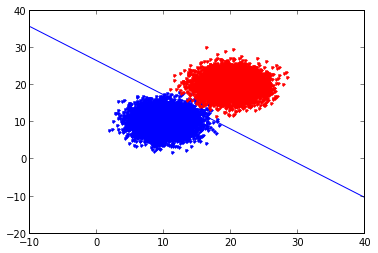
\includegraphics[width=0.7\textwidth]{stat_hadoop_logreg_files/stat_hadoop_logreg_fig_01.png}
\par
\end{center}
\end{codeoutput}
\end{codecell}
Kaynaklar

{[}1{]}
http://alex.smola.org/teaching/berkeley2012/slides/4\_Optimization.pdf

{[}2{]}
http://cs.kangwon.ac.kr/\ensuremath{\sim}ysmoon/courses/2011\_1/grad\_mining/slides/07-2.pdf

{[}3{]} http://www.slideshare.net/hadoop/modeling-with-hadoop-kdd2011

{[}4{]}
http://www.xmarks.com/site/www.cs.stanford.edu/people/ang/papers/nips06-mapreducemulticore.pdf

{[}5{]} http://books.nips.cc/papersnips23/NIPS2010\_1162.pdf

{[}6{]} http://simianer.de/P12-1002-slides.pdf

{[}7{]}
http://www.holehouse.org/mlclass/17\_Large\_Scale\_Machine\_Learning.html

{[}8{]}
https://github.com/elsevierlabs/logistic-regression-sgd-mapreduce

\end{document}
